\documentclass[11pt,a4paper]{article}
\usepackage[T1]{fontenc}
\usepackage[utf8]{inputenc}
\usepackage{lmodern}
\usepackage{microtype}
\usepackage[a4paper,margin=23mm]{geometry}
\usepackage{amsmath,amssymb,bm,mathtools}
\usepackage{siunitx}
\usepackage{graphicx}
\usepackage{booktabs,longtable,array}
\usepackage{caption,subcaption}
\usepackage{tikz}
\usepackage{xcolor}
\usepackage{enumitem}
\usepackage{natbib}
\usepackage[hidelinks]{hyperref}
\graphicspath{{figures/}}
\sisetup{separate-uncertainty=true}

\newcommand{\rhoA}{\rho_{\mathrm{afterSRC}}}
\newcommand{\rhoS}{\rho_{\mathrm{preSAMURAI}}}
\newcommand{\pt}{p_T}
\newcommand{\Tr}{\operatorname{Tr}}
\newcommand{\dd}{\mathrm{d}}
\newcommand{\R}{\mathsf{R}}
\newcommand{\T}{\mathsf{P}}

\title{Transport of a Tensor-Polarized Deuteron Beam\\from Downstream of SRC to the SAMURAI Experimental Area}
\author{Polarimeter spin-transport working note}
\date{24 August 2026}

\begin{document}
\maketitle

\begin{abstract}
This note develops a density-matrix treatment of a spin-1 deuteron beam transported from a polarimeter downstream of the RIKEN Superconducting Ring Cyclotron (SRC) to a second polarimeter in front of SAMURAI.  It uses the Cartesian tensor-polarization convention already used by this repository and the measured $d$--$p$ analyzing-power tables at \SI{190}{MeV/u}.  Deterministic magnetic transport is unitary: it rotates the vector and rank-2 tensor polarization without changing the density-matrix eigenvalues or purity.  In an ideal horizontal dipole, a vertical axial tensor state is invariant, whereas an initially longitudinal axial tensor develops $p_{xx}$ and $p_{xz}$ components in the transported beam frame.  From 2022 CODATA constants, a \SI{380}{MeV} deuteron has $\gamma=1.20260044$, $G_d=-0.14298727$, and $G_d\gamma=-0.17195655$.  Thus its spin rotates relative to the momentum by $-0.17195655$ times a signed ideal-dipole orbit bend.  The two proposed polarimeters can test a constrained spin-transfer model and can separate coherent axis rotation from loss of tensor magnitude, but a general density matrix or arbitrary three-dimensional transfer cannot be reconstructed from four sectors without additional polarization modes, angular channels, calibration, and beam tracking.  No complete, sourceable SRC-to-pre-SAMURAI magnet sequence and setting file was found; all numerical bend examples in this note are therefore explicitly illustrative.
\end{abstract}

\begin{center}
\fcolorbox{black}{gray!8}{\parbox{0.88\textwidth}{\centering\Large
$\boxed{\text{rotation of the polarization tensor}\;\neq\;\text{loss of polarization}}$}}
\end{center}

\tableofcontents
\clearpage

\section{Motivation and scope}

The experimental question is not merely whether a polarization number is nonzero.  It is whether the tensor state measured downstream of SRC is transported into a known tensor state at the SAMURAI target.  For coherent transport,
\begin{equation}
 \boxed{\rhoS=U_{\mathrm{SRC\to SAMURAI}}\,\rhoA\,
 U_{\mathrm{SRC\to SAMURAI}}^\dagger}. \label{eq:central}
\end{equation}
The distinction between a laboratory-fixed axis, the initial beam axis, and the transported local beam axis is essential.  A state that is longitudinal upstream is not automatically longitudinal downstream when the momentum bends.

\begin{figure}[htbp]
 \centering
 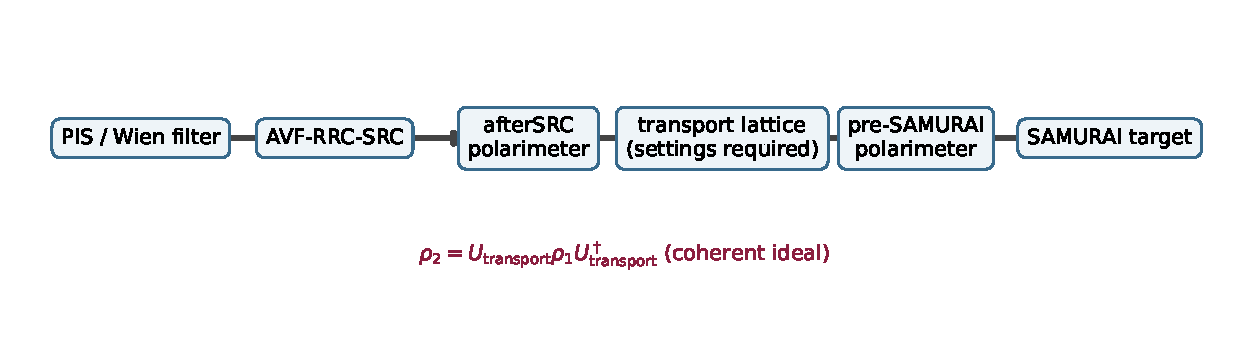
\includegraphics[width=\textwidth]{01_beamline_concept.pdf}
 \caption{Central experimental chain.  The two polarimeters bracket the unknown transport lattice.  Magnet names, field maps, signed bends, and optics settings are required before Eq.~\eqref{eq:central} becomes a RIKEN-specific prediction.}
 \label{fig:beamline}
\end{figure}

The RIKEN polarized ion source (PIS) can prepare vector and tensor spin modes; a Wien filter downstream of its ionizer controls the spin orientation before AVF injection.  Polarized deuterons have been accelerated through the AVF--RRC--SRC cascade at nominal \SIlist{190;250;300}{MeV/u}, and typical polarization is reported as roughly 80\% of the ideal mode value \citep{Sakamoto2016}.  This establishes the source and acceleration context, but it does not supply the element-by-element spin-transfer map between the proposed afterSRC and pre-SAMURAI stations.

The \SI{30}{degree} SAMURAI configuration discussed in the experiment simulation is a spectrometer configuration downstream of the experimental target.  It must not be substituted for an upstream SRC-to-SAMURAI beam bend.  The SAMURAI magnet specifications and upstream beam detectors are documented \citep{Kobayashi2013,RIKENSAMURAI}, but the transport relevant here terminates at the target before that analyzing magnet.

\section{Spin-1 density matrix and repository normalization}

\subsection{Operators and expansion}

In the ordered $S_z$ basis $\{|+1\rangle,|0\rangle,|-1\rangle\}$, with dimensionless spin matrices,
\begin{equation}
 S_x=\frac{1}{\sqrt2}\begin{pmatrix}0&1&0\\1&0&1\\0&1&0\end{pmatrix},\quad
 S_y=\frac{1}{\sqrt2}\begin{pmatrix}0&-i&0\\i&0&-i\\0&i&0\end{pmatrix},\quad
 S_z=\begin{pmatrix}1&0&0\\0&0&0\\0&0&-1\end{pmatrix}.
\end{equation}
Following the Cartesian convention used in the existing polarimeter note and in the standard review by \citet{Ohlsen1972}, define
\begin{equation}
 Q_{ij}=\frac{3}{2}(S_iS_j+S_jS_i)-2\delta_{ij}I,
 \qquad p_i=\Tr(\rho S_i),\qquad p_{ij}=\Tr(\rho Q_{ij}). \label{eq:operators}
\end{equation}
The tensor is real, symmetric, and traceless:
\begin{equation}
 p_{ij}=p_{ji},\qquad p_{xx}+p_{yy}+p_{zz}=0. \label{eq:tracefree}
\end{equation}
The repository expansion is
\begin{align}
 \rho={}&\frac{I}{3}+\frac12\sum_i p_iS_i
 +\frac19\sum_i p_{ii}Q_{ii}
 +\frac29\sum_{i<j}p_{ij}Q_{ij}. \label{eq:rhoexpand}
\end{align}
Equation~\eqref{eq:rhoexpand} is the implemented normalization; no new $p_{ij}$ convention is introduced in this work.

\subsection{Magnetic-substate populations and allowed range}

For a quantization axis $a$, a state diagonal in $m_a$ has populations $N_{+1},N_0,N_{-1}$ with unit sum.  The repository convention gives
\begin{equation}
 p_a=N_{+1}-N_{-1},\qquad
 p_{aa}=N_{+1}+N_{-1}-2N_0=1-3N_0. \label{eq:popdef}
\end{equation}
Therefore
\begin{equation}
 N_0=\frac{1-p_{aa}}{3},\quad
 N_{+1}=\frac{2+p_{aa}+3p_a}{6},\quad
 N_{-1}=\frac{2+p_{aa}-3p_a}{6}. \label{eq:pops}
\end{equation}
For zero vector polarization, positivity gives
\begin{equation}
 -2\le p_{aa}\le 1. \label{eq:range}
\end{equation}
Thus ``80\% tensor polarization'' must be tied to a mode and convention.  The illustrative value $p_{aa}=0.8$ is physical, but a source mode near the negative extreme can have $p_{aa}<-1$.  Recent RIBF recovery measurements report, for example, $p_{yy}=-0.741\pm0.039$ and $p_{yy}=0.565\pm0.052$ in different PIS modes \citep{RIKENAPR58Polarization}.

\section{Explicit initial $p_{zz}$ and $p_{yy}$ states}

An axially symmetric tensor of magnitude $\pt$ and principal axis $\hat{\bm n}$ is
\begin{equation}
 \T(\hat{\bm n},\pt)=\frac32\pt\,\hat{\bm n}\hat{\bm n}^{\mathsf T}-\frac12\pt I. \label{eq:axialtensor}
\end{equation}
Its eigenvalues are $(-\pt/2,-\pt/2,\pt)$.  The magnitude and axis are separate parameters.  Relabeling the axis from $z$ to $y$ rotates the same eigenvalue spectrum; it does not define a different unit of polarization.

\subsection{Longitudinal axial state}

For $\hat{\bm n}=\hat z$ and zero vector polarization,
\begin{equation}
 \T_z^{(0)}=\begin{pmatrix}-\pt/2&0&0\\0&-\pt/2&0\\0&0&\pt\end{pmatrix},\qquad
 \rho_{zz}^{(0)}=\begin{pmatrix}
 (2+\pt)/6&0&0\\0&(1-\pt)/3&0\\0&0&(2+\pt)/6
 \end{pmatrix}. \label{eq:rhoz}
\end{equation}
Hence $p_{xx}=p_{yy}=-p_{zz}/2$.  At $\pt=0.8$,
\begin{equation}
 \rho_{zz}^{(0)}=\begin{pmatrix}0.4666667&0&0\\0&0.0666667&0\\0&0&0.4666667\end{pmatrix}.
\end{equation}

\begin{figure}[htbp]
 \centering
 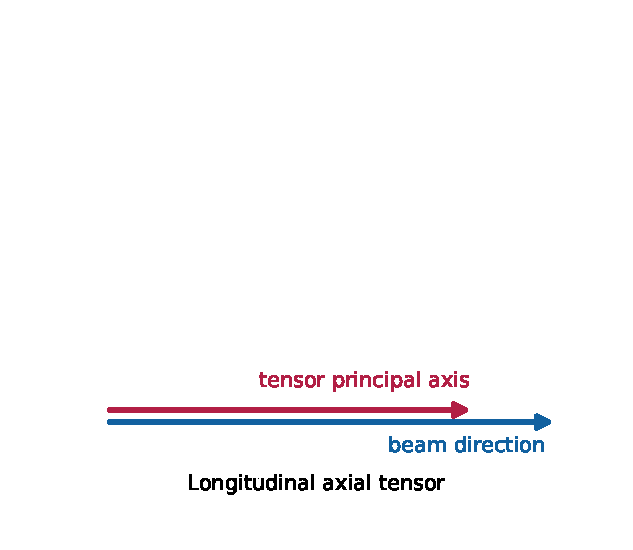
\includegraphics[width=0.72\textwidth]{06_initial_pzz.pdf}
 \caption{Initial longitudinal axial tensor.  The principal axis is parallel to the initial beam direction.}
\end{figure}

\subsection{Vertical axial state}

For $\hat{\bm n}=\hat y$,
\begin{equation}
 \T_y^{(0)}=\begin{pmatrix}-\pt/2&0&0\\0&\pt&0\\0&0&-\pt/2\end{pmatrix},
\end{equation}
and in the same $S_z$ magnetic-substate basis,
\begin{equation}
 \rho_{yy}^{(0)}=\begin{pmatrix}
 \frac13-\frac{\pt}{12}&0&-\frac{\pt}{4}\\
 0&\frac13+\frac{\pt}{6}&0\\
 -\frac{\pt}{4}&0&\frac13-\frac{\pt}{12}
 \end{pmatrix}. \label{eq:rhoy}
\end{equation}
For $\pt=0.8$, this is
\begin{equation}
 \rho_{yy}^{(0)}=\begin{pmatrix}0.2666667&0&-0.2\\0&0.4666667&0\\-0.2&0&0.2666667\end{pmatrix}.
\end{equation}
The off-diagonal elements in Eq.~\eqref{eq:rhoy} are not decoherence; they appear because a state diagonal in $S_y$ is expressed in the $S_z$ basis.

\begin{figure}[htbp]
 \centering
 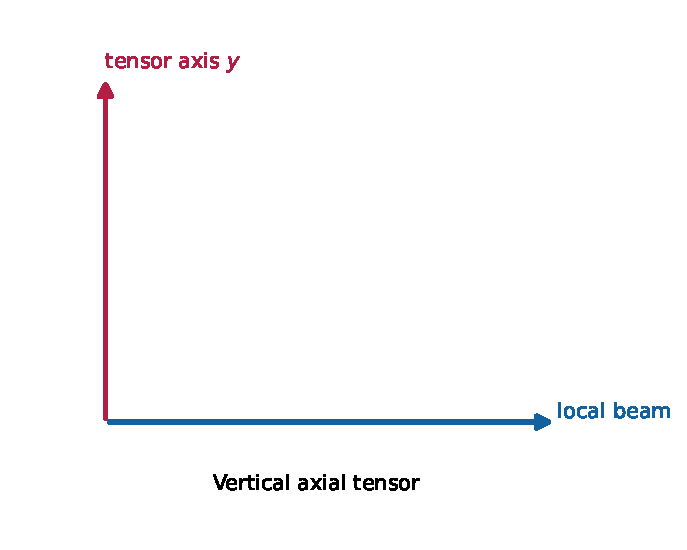
\includegraphics[width=0.72\textwidth]{04_initial_pyy.pdf}
 \caption{Initial vertical axial tensor.}
\end{figure}

\section{Unitary density-matrix evolution}

For a spin Hamiltonian $H_{\rm spin}$,
\begin{equation}
 i\hbar\frac{\dd\rho}{\dd t}=[H_{\rm spin},\rho],\qquad
 \rho_f=U\rho_iU^\dagger,
\end{equation}
with
\begin{equation}
 U=\mathcal T\exp\left[-\frac{i}{\hbar}\int H_{\rm spin}(t)\,\dd t\right]. \label{eq:unitary}
\end{equation}
When every particle experiences the same $U$,
\begin{equation}
 \Tr\rho=1,\quad \operatorname{eig}(\rho_f)=\operatorname{eig}(\rho_i),\quad
 \Tr\rho_f^2=\Tr\rho_i^2. \label{eq:invariants}
\end{equation}
Therefore deterministic bending is coherent spin rotation, not automatic depolarization.  Nonunitary changes can arise after averaging particles with different $U$, from spin-dependent loss, or from interactions not included in a pure magnetic-dipole Hamiltonian.

For a spatial rotation $\R$,
\begin{equation}
 p_i'=R_{ij}p_j,\qquad \T'=\R\T\R^{\mathsf T},\qquad
 \rho'=D^{(1)}(\R)\rho D^{(1)}(\R)^\dagger. \label{eq:rotlaws}
\end{equation}
The accompanying code verifies numerically, to $10^{-12}$, that the two tensor transformations in Eq.~\eqref{eq:rotlaws} agree for general axes and physical density matrices.

\section{Thomas--BMT transport for the deuteron}

The Thomas--Bargmann--Michel--Telegdi equation \citep{Bargmann1959} for the rest-frame spin vector in laboratory time is
\begin{equation}
 \frac{\dd\bm s}{\dd t}=\bm\Omega_s\times\bm s,
\end{equation}
\begin{align}
 \bm\Omega_s=-\frac{q}{m}\bigg[&\left(G+\frac1\gamma\right)\bm B
 -\frac{G\gamma}{\gamma+1}\bm\beta(\bm\beta\cdot\bm B) \notag\\
 &-\left(G+\frac1{\gamma+1}\right)\frac{\bm\beta\times\bm E}{c}\bigg]. \label{eq:bmt}
\end{align}
Here $G=(g-2)/2$, where $g$ is defined using the transported particle mass: $\bm\mu=g(q/2m)\bm S$.  CODATA gives \citep{Mohr2025CODATA}
\begin{align}
 \frac{\mu_d}{\mu_N}&=0.8574382335(22), &
 \frac{m_d}{m_p}&=1.9990075012699(84),\\
 m_dc^2&=\SI{1875.61294500(58)}{MeV}. &&
\end{align}
The first number is often called the deuteron nuclear $g$-factor, but it is not directly the BMT $g$ because $\mu_N=e\hbar/(2m_p)$.  Consequently,
\begin{align}
 g_{d,\rm BMT}&=\frac{\mu_d}{\mu_N}\frac{m_d}{m_p}=1.71402546064,\\
 G_d&=\frac{g_{d,\rm BMT}-2}{2}=-0.14298726968. \label{eq:Gd}
\end{align}
For total deuteron kinetic energy $T_d=\SI{380}{MeV}$,
\begin{equation}
 \gamma=1+\frac{T_d}{m_dc^2}=1.20260043577,\qquad
 G_d\gamma=-0.17195655283. \label{eq:Ggamma}
\end{equation}

Equation~\eqref{eq:bmt} is a magnetic-dipole transport equation.  A complete high-precision lattice treatment should also assess electric quadrupole interactions in strong field gradients, fringe fields, material interactions, and spin-dependent aperture losses.  Those effects are not inferred from a reference trajectory alone.

\section{Orbital bending versus spin bending}

Consider $\bm E=0$ and $\bm B\perp\bm\beta$.  The signed angular velocities about the field axis are
\begin{equation}
 \omega_{\rm orbit}=-\frac{qB}{\gamma m},\qquad
 \omega_{\rm spin}=-\frac{qB}{m}\left(G+\frac1\gamma\right).
\end{equation}
Therefore, for a signed orbit bend $\theta$,
\begin{equation}
 \psi_{\rm spin}^{\rm lab}=(1+G\gamma)\theta,\qquad
 \boxed{\delta\equiv\psi_{\rm spin}^{\rm lab}-\theta=G\gamma\theta}. \label{eq:relative}
\end{equation}
Changing the sign convention for the bend reverses all three signed angles; the measurable statement is the relative orientation defined in Eq.~\eqref{eq:relative}.

\begin{figure}[htbp]
 \centering
 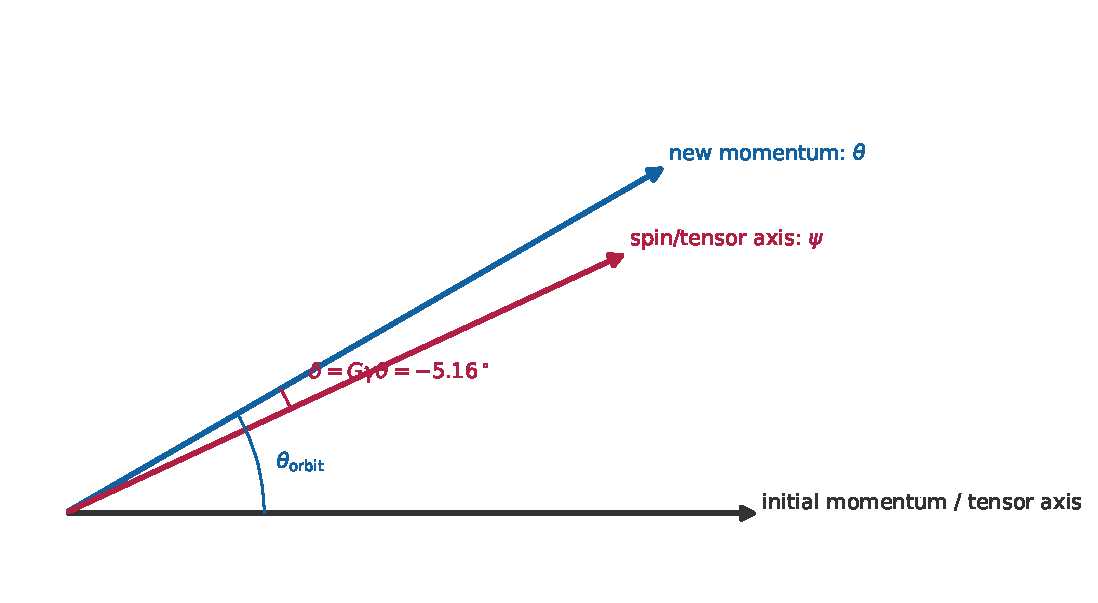
\includegraphics[width=0.78\textwidth]{02_orbit_vs_spin.pdf}
 \caption{Illustrative \SI{30}{degree} single horizontal dipole.  Momentum and spin rotate in the laboratory by different angles.  This is not a claim about the SRC-to-SAMURAI net bend.}
 \label{fig:orbitspin}
\end{figure}

\begin{table}[htbp]
 \centering
 \caption{Illustrative ideal-dipole spin rotation for a \SI{380}{MeV} deuteron.  Values are signed for positive $\theta$ in the convention of Eq.~\eqref{eq:relative}.}
 \begin{tabular}{rrr}
 \toprule
 Orbit bend & Spin rotation in lab & Spin relative to beam $\delta$\\
 \midrule
 \SI{1}{degree}  & \SI{0.828043}{degree} & \SI{-0.171957}{degree}\\
 \SI{3}{degree}  & \SI{2.484130}{degree} & \SI{-0.515870}{degree}\\
 \SI{5}{degree}  & \SI{4.140217}{degree} & \SI{-0.859783}{degree}\\
 \SI{10}{degree} & \SI{8.280434}{degree} & \SI{-1.719566}{degree}\\
 \SI{20}{degree} & \SI{16.560869}{degree} & \SI{-3.439131}{degree}\\
 \SI{30}{degree} & \SI{24.841303}{degree} & \SI{-5.158697}{degree}\\
 \bottomrule
 \end{tabular}
 \label{tab:bends}
\end{table}

\section{Coordinate systems}

Three frames are used:
\begin{description}[style=nextline]
 \item[Laboratory frame $(x_{\rm lab},y_{\rm lab},z_{\rm lab})$] Fixed to the hall.
 \item[Initial beam frame $(x_0,y_0,z_0)$] $z_0$ is the reference direction at afterSRC.
 \item[Local beam frame $(x_b,y_b,z_b)$] $z_b$ follows the transported reference momentum and defines the polarimeter scattering angles.
\end{description}
If $\R_o$ transports the orbit frame and $\R_s$ transports the spin in the lab, the effective spin rotation seen by the downstream polarimeter is
\begin{equation}
 \R_{\rm rel}=\R_o^{\mathsf T}\R_s. \label{eq:relmatrix}
\end{equation}

\begin{figure}[htbp]
 \centering
 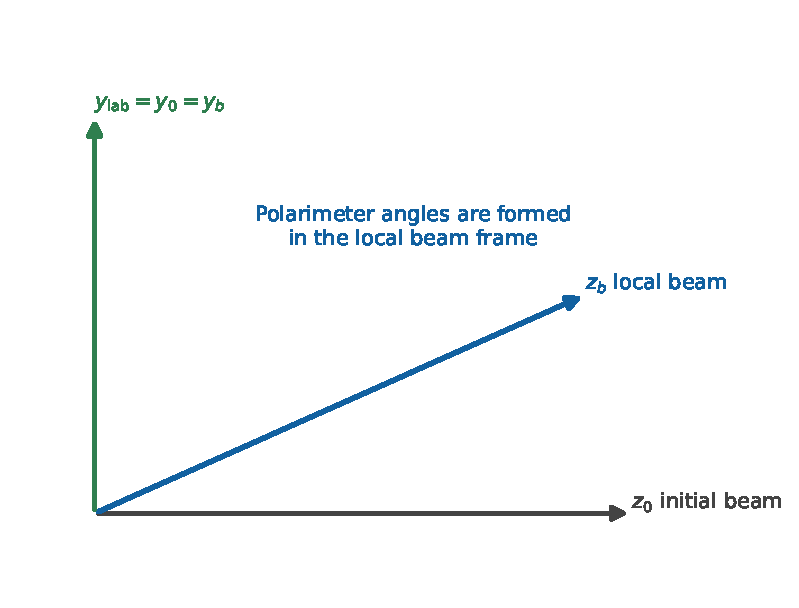
\includegraphics[width=0.72\textwidth]{03_coordinate_frames.pdf}
 \caption{The downstream polarimeter uses the local incident-beam frame, not the initial or hall frame.}
\end{figure}

\section{Ideal horizontal bending}

Let $\bm B\parallel\hat y$ and the orbit bend in the $xz$ plane.  In the local beam frame the tensor undergoes $\R_y(\delta)$.

\subsection{Initially vertical $p_{yy}$}

For $\T_y^{(0)}=\operatorname{diag}(-\pt/2,\pt,-\pt/2)$,
\begin{equation}
 \R_y(\delta)\T_y^{(0)}\R_y^{\mathsf T}(\delta)=\T_y^{(0)}. \label{eq:pyyinvariant}
\end{equation}
Thus $p_{yy}'=p_{yy}$, $p_{xx}'=p_{zz}'=-p_{yy}/2$, and all off-diagonal components remain zero.  The entire density matrix is unchanged, not only one component.

\begin{figure}[htbp]
 \centering
 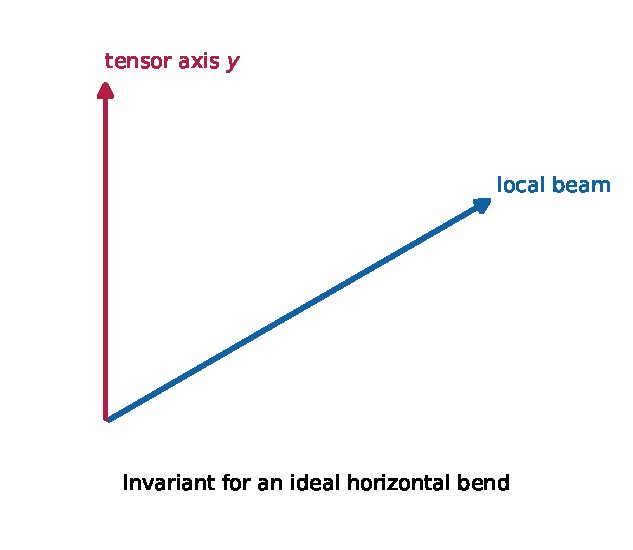
\includegraphics[width=0.72\textwidth]{05_transported_pyy.pdf}
 \caption{Vertical axial tensor after an ideal horizontal bend.  Its axis coincides with the bend and BMT-precession axis.}
\end{figure}

This invariance is not universal.  Vertical steering, radial or longitudinal fields, nonplanar bends, solenoids, quadrupole and fringe fields, a downstream Wien filter, or transverse coupling can rotate the tensor away from $y$.  The actual lattice must be evaluated as a three-dimensional ordered product.

\subsection{Initially longitudinal $p_{zz}$}

For the state in Eq.~\eqref{eq:rhoz}, direct multiplication gives
\begin{align}
 p_{xx}'&=\pt\left(\sin^2\delta-\frac12\cos^2\delta\right),\\
 p_{yy}'&=-\frac12\pt,\\
 p_{zz}'&=\pt\left(\cos^2\delta-\frac12\sin^2\delta\right)
          =\pt\left(\frac14+\frac34\cos2\delta\right),\\
 p_{xz}'&=\frac32\pt\sin\delta\cos\delta
          =\frac34\pt\sin2\delta. \label{eq:pzzrotate}
\end{align}
The sign of $p_{xz}'$ follows the stated active-rotation convention.  An initially longitudinal tensor has not vanished: its principal axis has rotated relative to $z_b$, redistributing its Cartesian components.

For the illustrative $\pt=0.8$, $\theta=+\SI{30}{degree}$ case, $\delta=-\SI{5.158697}{degree}$ and
\begin{equation}
 \T_b=\begin{pmatrix}
 -0.390298&0&-0.107461\\0&-0.400000&0\\-0.107461&0&0.790298
 \end{pmatrix}. \label{eq:numerictensor}
\end{equation}
In the $S_{z_b}$ basis,
\begin{equation}
 \rho_b=\begin{pmatrix}
 0.465050&-0.025329&0.001617\\
 -0.025329&0.069901&0.025329\\
 0.001617&0.025329&0.465050
 \end{pmatrix}. \label{eq:numericrho}
\end{equation}
It has the same eigenvalues $(0.466667,0.466667,0.066667)$ and the same purity as Eq.~\eqref{eq:rhoz}.

\begin{figure}[htbp]
 \centering
 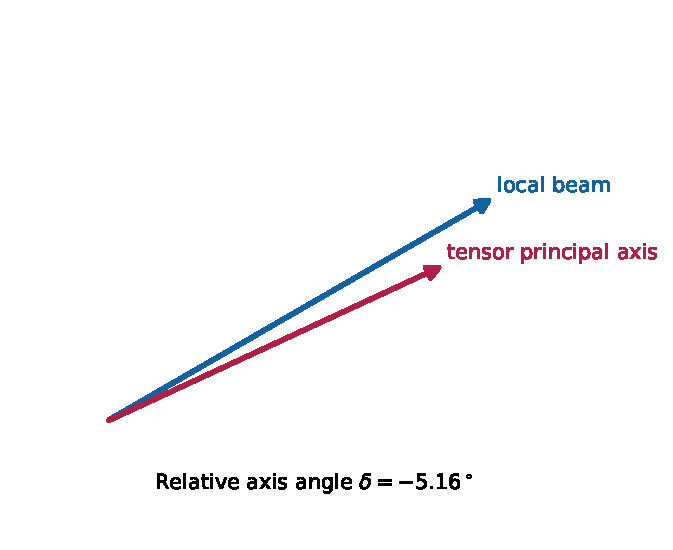
\includegraphics[width=0.72\textwidth]{07_transported_pzz.pdf}
 \caption{An initially longitudinal tensor after the illustrative bend.  The principal axis is no longer parallel to the local momentum.}
\end{figure}

\begin{figure}[htbp]
 \centering
 \begin{subfigure}{0.49\textwidth}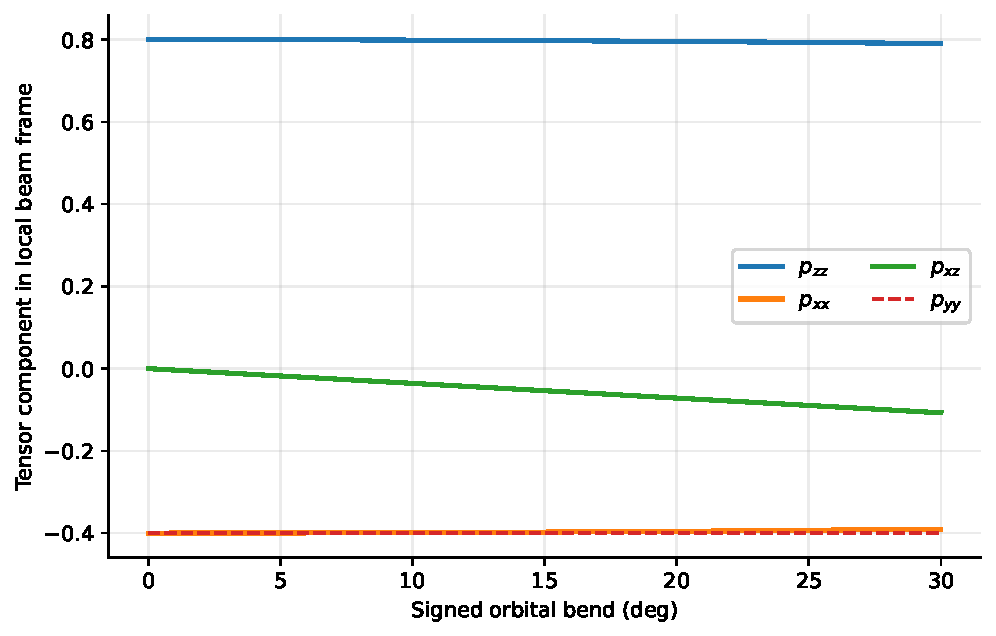
\includegraphics[width=\linewidth]{08_tensor_components_vs_bend.pdf}\end{subfigure}
 \begin{subfigure}{0.49\textwidth}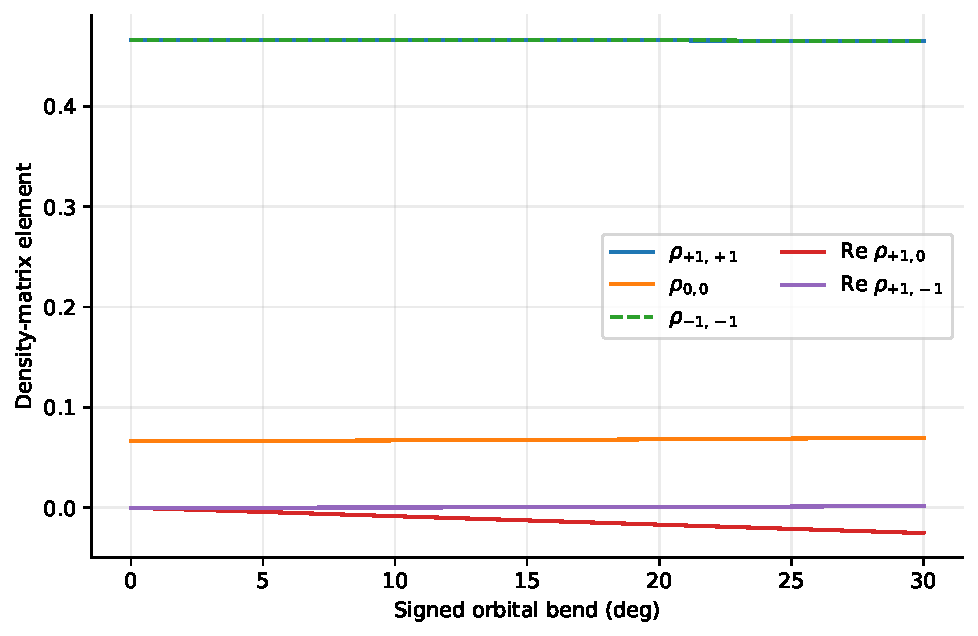
\includegraphics[width=\linewidth]{09_density_matrix_vs_bend.pdf}\end{subfigure}
 \caption{Illustrative single-dipole scan for $\pt=0.8$.  Left: tensor components in the local beam frame.  Right: density-matrix elements in the same frame.}
\end{figure}

\section{General multi-magnet transport and transfer matrix}

For ordered elements,
\begin{equation}
 \R_s^{\rm total}=\R_{s,N}\cdots\R_{s,2}\R_{s,1},\qquad
 \R_o^{\rm total}=\R_{o,N}\cdots\R_{o,2}\R_{o,1}. \label{eq:chain}
\end{equation}
Rotations do not generally commute; replacing a nonplanar lattice by a scalar net bend can be wrong.  The accompanying code reads YAML/JSON entries containing element name, type, signed bend axis and angle, energy, and an optional externally calculated spin angle.  The supplied example lattice is explicitly tagged as illustrative.

For a horizontal relative rotation, define
\begin{equation}
 \bm t=(p_{xx}-p_{yy},\ p_{zz},\ p_{xz},\ p_{yz},\ p_{xy})^{\mathsf T}.
\end{equation}
Then $\bm t'=M_y(\delta)\bm t$, where $c=\cos\delta$, $s=\sin\delta$ and
\begin{equation}
 M_y=\begin{pmatrix}
 (1+c^2)/2&3s^2/2&2sc&0&0\\
 s^2/2&c^2-s^2/2&-2sc&0&0\\
 -sc/2&3sc/2&c^2-s^2&0&0\\
 0&0&0&c&-s\\
 0&0&0&s&c
 \end{pmatrix}. \label{eq:transfermatrix}
\end{equation}
This provides a compact experiment-facing prediction from the upstream measured components to the downstream components.

\subsection{Status of the real SRC-to-SAMURAI lattice}

The repository and public sources establish the PIS--Wien--AVF--RRC--SRC polarized-deuteron chain \citep{Sakamoto2016}, BigRIPS/ZeroDegree/SAMURAI facility boundaries, and the presence of beam phase-space detectors upstream of SAMURAI \citep{RIKENSAMURAI}.  They do not provide a single sourceable file containing the magnet sequence, signed bend axes, field integrals or maps, energy history, and actual settings between the proposed afterSRC and pre-SAMURAI stations for this primary deuteron tune.  Consequently this note uses:
\begin{enumerate}
 \item Scenario A: one generic horizontal dipole, used for analytic checks;
 \item Scenario B: an ordered sequence when individual sourced bends become available;
 \item Scenario C: the current placeholder lattice, which refuses to claim a RIKEN-specific arrival state.
\end{enumerate}
The required machine input is listed in Sec.~\ref{sec:requirements}.

\section{Coherent rotation versus ensemble depolarization}

For beam phase-space coordinate $\xi$,
\begin{equation}
 \bar\rho_f=\int\dd\xi\,f(\xi)U(\xi)\rho_iU^\dagger(\xi), \label{eq:ensemble}
\end{equation}
which is generally not $U(\bar\xi)\rho_iU^\dagger(\bar\xi)$.  A spread of spin phases therefore reduces ensemble purity even though each particle evolves unitarily.

For an initially $z$-axial tensor and $\delta\sim\mathcal N(\bar\delta,\sigma_\delta)$ about $y$,
\begin{align}
 \langle p_{zz}\rangle&=\pt\left[\frac14+\frac34e^{-2\sigma_\delta^2}\cos(2\bar\delta)\right],\\
 \langle p_{xx}\rangle&=\pt\left[\frac14-\frac34e^{-2\sigma_\delta^2}\cos(2\bar\delta)\right],\\
 \langle p_{xz}\rangle&=\frac34\pt e^{-2\sigma_\delta^2}\sin(2\bar\delta),\\
 \langle p_{yy}\rangle&=-\frac12\pt. \label{eq:gaussian}
\end{align}
Only the harmonics that depend on the dispersed phase are damped.  A one-axis phase randomization does not necessarily make the ensemble isotropic.

\begin{figure}[htbp]
 \centering
 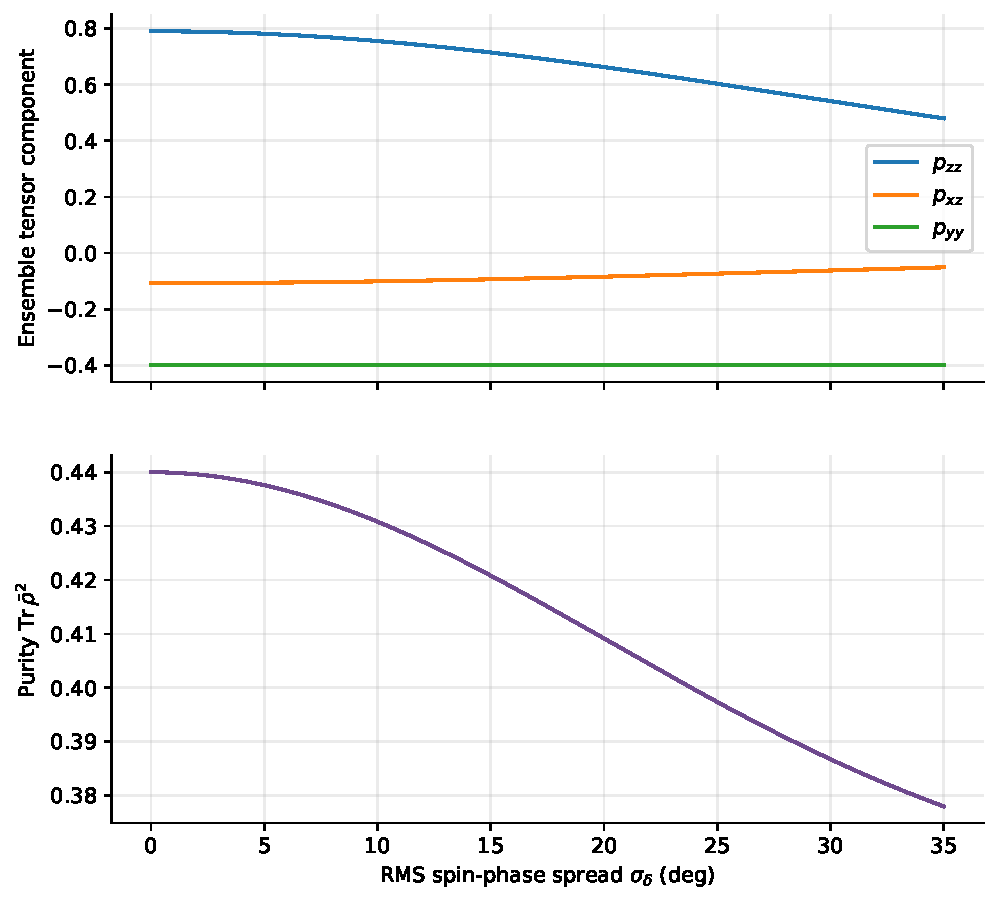
\includegraphics[width=0.8\textwidth]{12_coherent_rotation_vs_depolarization.pdf}
 \caption{Gaussian phase-spread example.  At zero spread the change is coherent rotation; increasing spread lowers $\Tr\bar\rho^2$ and damps phase-sensitive tensor components.}
\end{figure}

\section{What the polarimeters measure}

The polarimeters do not directly read all matrix elements.  They record $d+p\to d+p$ yields.  In the local incident-beam frame, the repository cross-section convention is
\begin{align}
 \frac{\sigma(\theta,\phi)}{\sigma_0(\theta)}={}&1
 +\frac32(p_x\sin\phi+p_y\cos\phi)A_y
 +\frac23(p_{xz}\cos\phi-p_{yz}\sin\phi)A_{xz}\notag\\
 &+\frac16\left[(p_{xx}-p_{yy})\cos2\phi-2p_{xy}\sin2\phi\right](A_{xx}-A_{yy})
 +\frac12p_{zz}A_{zz}. \label{eq:crosssection}
\end{align}
For the measured spherical observables in the repository table \citep{Sekiguchi2017},
\begin{equation}
 A_y=\frac{2}{\sqrt3}iT_{11},\quad A_{xz}=-\sqrt3T_{21},\quad
 A_{xx}-A_{yy}=2\sqrt3T_{22},\quad A_{zz}=\sqrt2T_{20}. \label{eq:conversion}
\end{equation}
At $\theta_{\rm cm}=\SI{68.6}{degree}$ the interpolated values are
\begin{equation}
 A_{xz}=0.27540,\quad A_{xx}-A_{yy}=-1.16047,\quad A_{zz}=0.21355.
\end{equation}
Thus the transported $p_{xz}$ in Eq.~\eqref{eq:pzzrotate} produces a first-harmonic left--right signal, which is linear in small $\delta$.

\subsection{Normalization audit}

The C++ count implementation uses
\begin{align}
 f_{p_{zz}}&=1+\frac{\sqrt2}{2}T_{20}p_{zz},\\
 f_{LR/UD}&=1\mp\frac{\sqrt3}{2}T_{22}p_{yy}-\frac{\sqrt2}{4}T_{20}p_{yy}.
\end{align}
These agree with Eqs.~\eqref{eq:crosssection}--\eqref{eq:conversion} for an axial vertical tensor, $p_{xx}=p_{zz}=-p_{yy}/2$.  However, the displayed closed-form $R_{LRUD}$ inversion in the older \texttt{polarimeter\_stastic.tex} contains a factor-of-two discrepancy in its $A_{zz}$ denominator.  From the implemented sector factors,
\begin{equation}
 R_{LRUD}=\frac{N_L+N_R-N_U-N_D}{N_L+N_R+N_U+N_D}
 =-\frac{p_{yy}(A_{xx}-A_{yy})}{4-p_{yy}A_{zz}}, \label{eq:lrudaudit}
\end{equation}
not $-p_{yy}(A_{xx}-A_{yy})/(4-2p_{yy}A_{zz})$.  This note and its tests follow the code and the general cross section.  The older document should be corrected before its analytic inversion is used on data.

\subsection{Four-sector observability}

At $\phi=(0,\pi/2,\pi,3\pi/2)$,
\begin{align}
 N_L-N_R&\propto\frac43p_{xz}A_{xz},\\
 N_U-N_D&\propto-\frac43p_{yz}A_{xz},\\
 N_L+N_R-N_U-N_D&\propto\frac23(p_{xx}-p_{yy})(A_{xx}-A_{yy}). \label{eq:harmonics}
\end{align}
The total and multi-angle ratios constrain $p_{zz}$ through $A_{zz}$.  For an initially longitudinal axial model, $L-R$ is the leading small-angle observable for $\delta$; $LR-UD$ and multi-angle totals constrain $\pt$ and the even dependence on $\delta$.

\begin{figure}[htbp]
 \centering
 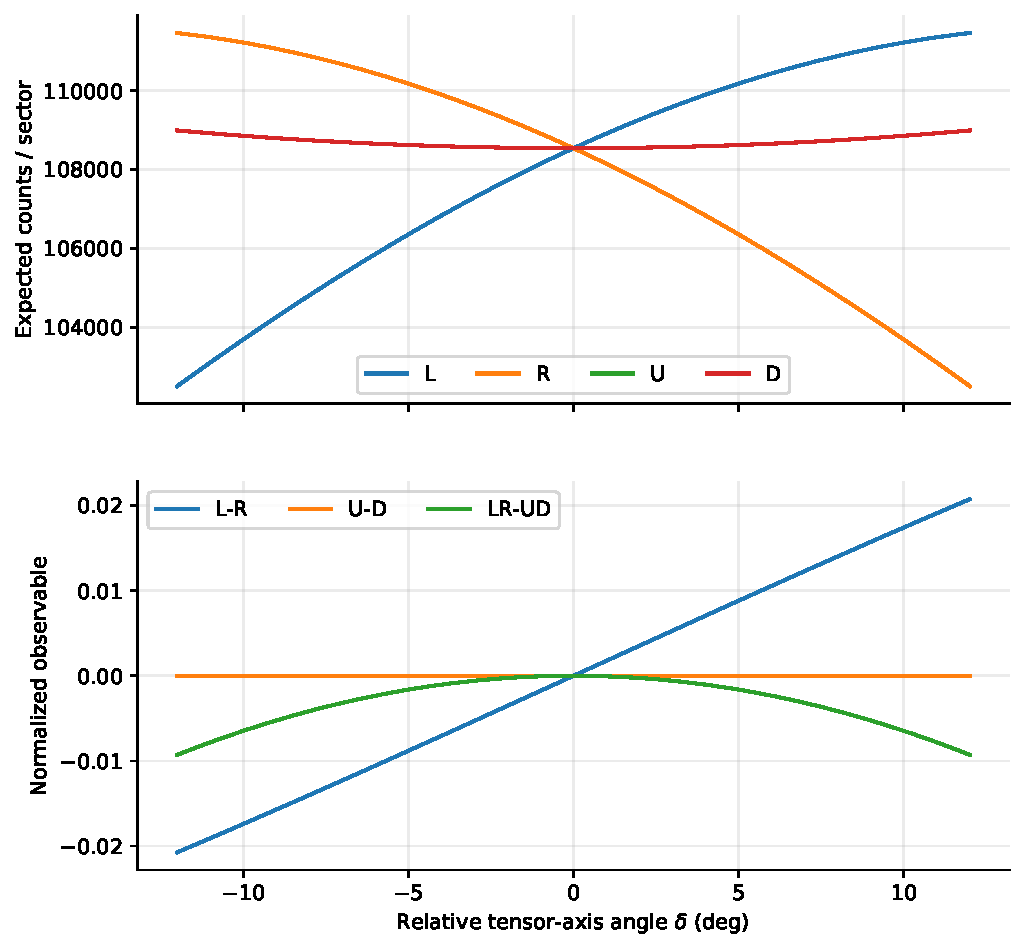
\includegraphics[width=0.82\textwidth]{10_four_sector_yields_vs_spin_angle.pdf}
 \caption{Point-detector yields at \SI{68.6}{degree} c.m. for a $\pt=0.8$ longitudinal axial state rotated about $y$.  The odd $L-R$ signal is the principal angle discriminator.}
\end{figure}

\section{Can two polarimeters reconstruct the spin transfer?}

The answer depends on the assumed state space.
\begin{itemize}
 \item \textbf{Planar axial model: yes, in principle.}  Fit a common $\pt$, relative axis angle $\delta$, and normalization to several angular channels.  Measure these parameters at afterSRC and pre-SAMURAI; their difference tests the predicted planar spin transfer.
 \item \textbf{General rank-2 tensor: not from one four-sector ring alone.}  A real symmetric traceless tensor has five independent components.  Vector polarization adds three.  Detector efficiencies and normalizations add nuisance parameters.
 \item \textbf{General three-dimensional transfer: additional inputs are required.}  Several noncollinear prepared spin modes, nonzero relevant analyzing powers, multiple scattering angles, calibrated sector efficiencies, and beam tracking are needed to identify a general $SO(3)$ spin rotation and distinguish it from ensemble depolarization.
\end{itemize}

The implemented Fisher calculation uses the compact detector's proton channels at \SI{53.4}{degree} and \SI{11.2}{degree} lab, corresponding to \SI{68.676}{degree} and \SI{155.703}{degree} c.m. at \SI{380}{MeV}, with relative rates from the repository cross-section table and point-detector solid angles.  With an illustrative unpolarized normalization of $10^5$ counts per forward sector, fixed analyzing powers, ideal efficiencies, and $\pt=0.8$, $\delta=-\SI{5.159}{degree}$, the statistical Fisher estimates are approximately
\begin{equation}
 \sigma(\pt)\simeq0.0063,\qquad \sigma(\delta)\simeq\SI{0.195}{degree}. \label{eq:fisher}
\end{equation}
They scale as $N^{-1/2}$.  These are sensitivity demonstrations, not forecasts: analyzing-power covariance, background, finite acceptance, efficiency calibration, beam nuisance parameters, and phase spread are omitted.

\begin{figure}[htbp]
 \centering
 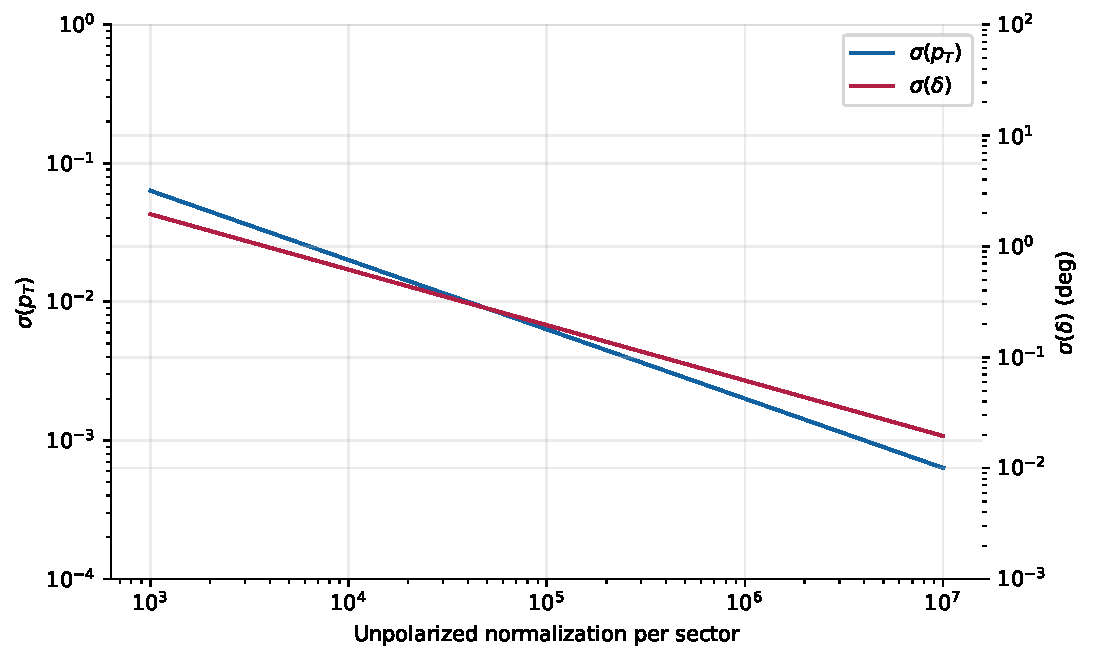
\includegraphics[width=0.8\textwidth]{11_tensor_axis_sensitivity.pdf}
 \caption{Statistical Fisher sensitivity of the two-channel axial fit under the stated ideal assumptions.}
\end{figure}

\begin{figure}[htbp]
 \centering
 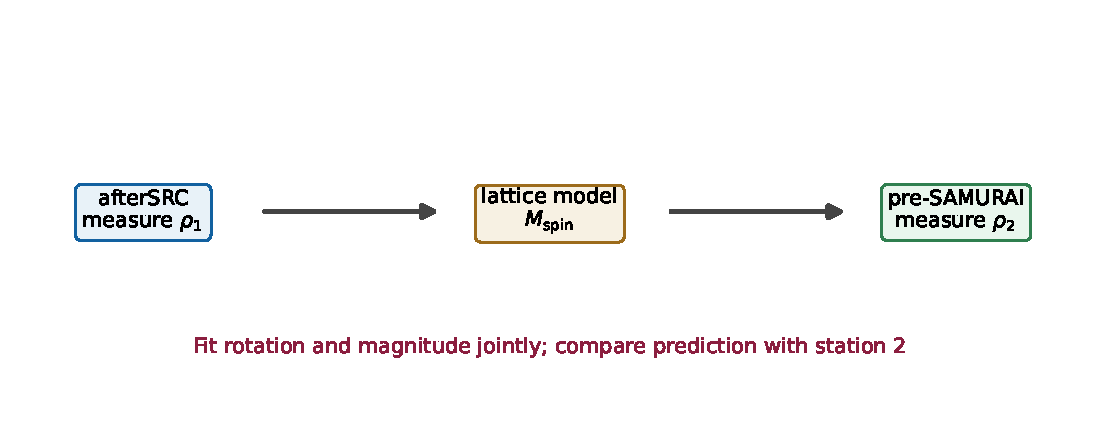
\includegraphics[width=0.88\textwidth]{14_two_polarimeter_spin_transfer.pdf}
 \caption{Experimental comparison.  Agreement tests the coherent transfer model; a reduced fitted magnitude with broadened phase-sensitive observables suggests ensemble decoherence or other loss mechanisms.}
\end{figure}

\section{Beam position and angle systematics}

Physical spin transport and polarimeter mis-steering are distinct operations:
\begin{equation}
 \rho_i\xrightarrow{\text{BMT lattice}}\rho_{\rm pol}
 \xrightarrow{(x_b,y_b,\alpha_x,\alpha_y)}(\theta_k,\phi_k)\xrightarrow{d\text{-}p\text{ response}}N_k. \label{eq:ordering}
\end{equation}
The nuisance vector is
\begin{equation}
 \bm b=(x_b,y_b,\alpha_x,\alpha_y).
\end{equation}
For detector center $\bm r_k$, interaction point $\bm r_b=(x_b,y_b,0)$, and normalized beam direction $\hat z_b\propto(\alpha_x,\alpha_y,1)$, the code recomputes
\begin{equation}
 \cos\theta_k=\widehat{(\bm r_k-\bm r_b)}\cdot\hat z_b,\qquad
 \phi_k=\operatorname{atan2}\!\left(\hat r_k\cdot\hat y_b,\hat r_k\cdot\hat x_b\right),
\end{equation}
as well as the inverse-square point-detector solid angle, the c.m. angle, the tabulated unpolarized cross section, and the interpolated analyzing powers.

The requested position scans use $x_b,y_b=\pm0.5,\pm1,\pm2,\pm\SI{5}{mm}$.  The angle scans use $\alpha_x,\alpha_y=\pm0.1,\pm0.5,\pm1,\pm2,\pm\SI{5}{mrad}$.  Representative biases when the fit incorrectly assumes a centered beam are shown in Table~\ref{tab:steering}.  Values are model-dependent and should guide tracker-inclusive simulation, not directly set mechanical tolerances.

\begin{table}[htbp]
 \centering
 \caption{Representative point-detector nuisance biases for the two-channel axial fit.  Signs correspond to the code coordinates.}
 \label{tab:steering}
 \begin{tabular}{llrr}
 \toprule
 Mode & Unmodelled nuisance & $\Delta\pt$ & $\Delta\delta$\\
 \midrule
 $p_{zz}$ & $x_b=+\SI{1}{mm}$ & $-0.00374$ & $+\SI{0.391}{degree}$\\
 $p_{zz}$ & $\alpha_x=+\SI{1}{mrad}$ & $-0.00042$ & $-\SI{0.0613}{degree}$\\
 $p_{zz}$ & $y_b=+\SI{1}{mm}$ & $-0.00078$ & $+\SI{0.00084}{degree}$\\
 $p_{yy}$ & $y_b=+\SI{1}{mm}$ & $-0.00115$ & $-\SI{1.024}{degree}$\\
 $p_{yy}$ & $\alpha_y=+\SI{1}{mrad}$ & $-0.00019$ & $-\SI{0.0585}{degree}$\\
 \bottomrule
 \end{tabular}
\end{table}

\begin{figure}[htbp]
 \centering
 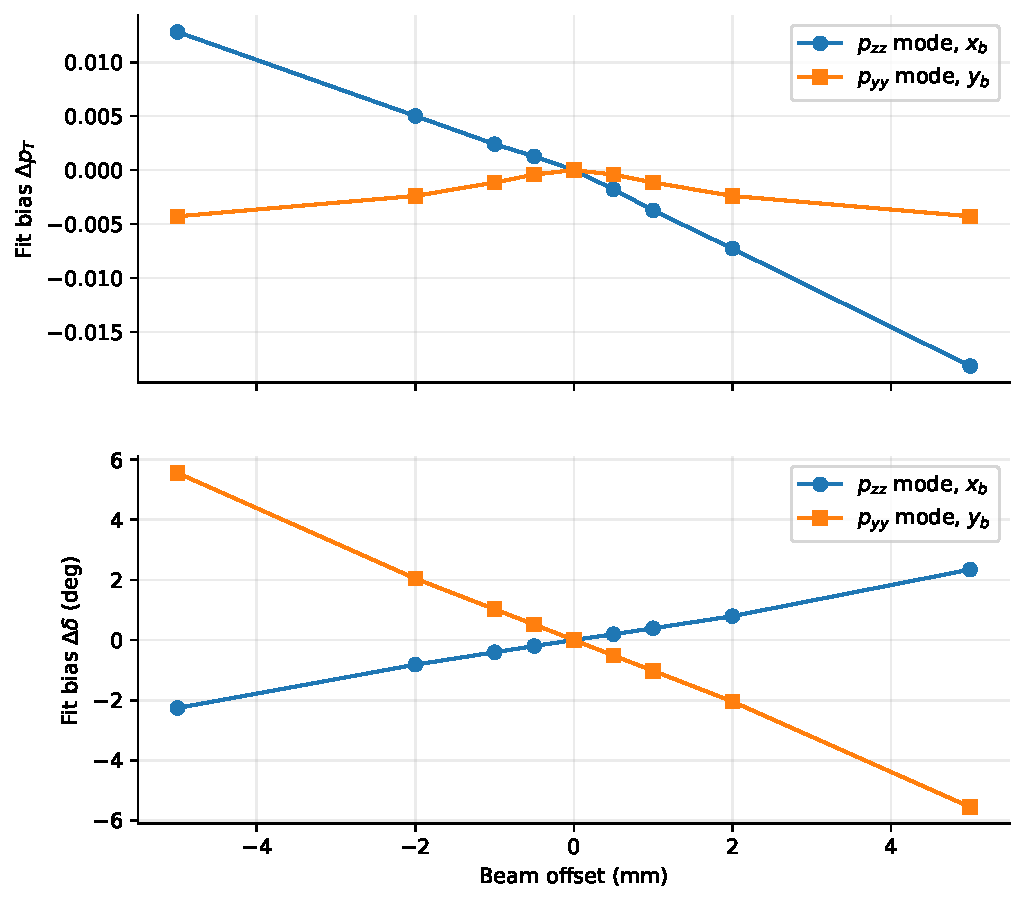
\includegraphics[width=0.8\textwidth]{13_beam_offset_fake_spin_rotation.pdf}
 \caption{Fitted bias versus beam offset in the point-detector model.  Horizontal offset most strongly mimics the $p_{zz}$ rotation signal; vertical offset most strongly mimics a tilt of the vertical axis.}
\end{figure}

Beam tracking at both polarimeters, reversal among source modes, unpolarized reference runs, sector-efficiency calibration, and a simultaneous likelihood in $(\pt,\delta,\bm b)$ are therefore part of a quantitative spin-transfer measurement.

\section{End-to-end synthetic scenarios}

The executable study script implements four reproducible demonstrations:
\begin{enumerate}
 \item $p_{yy}=0.8$ through an ideal horizontal bend: $\rho$ and all tensor components are invariant in the local beam frame.
 \item $p_{zz}=0.8$ through the same bend: $p_{xz}$ is generated and $L-R$ changes sign with $\delta$; the axial two-channel fit recovers magnitude and orientation for a centered beam.
 \item The same $p_{zz}$ state with Gaussian phase spread: phase-sensitive components and purity decrease according to Eq.~\eqref{eq:gaussian}.
 \item The same physical state with beam offset/angle: a fit that omits $\bm b$ returns biased $\pt$ and $\delta$, even though the input density matrix is unchanged.
\end{enumerate}
Generated CSV and JSON files preserve the numerical values behind the plots.

\section{Experimental requirements and missing information}\label{sec:requirements}

To turn the framework into a RIKEN-specific arrival-state prediction, obtain:
\begin{enumerate}
 \item the exact reference-trajectory path from afterSRC to the pre-SAMURAI target line for the polarized primary-deuteron tune;
 \item ordered magnet names and types, signed bend axes/angles, current settings, calibrated field integrals or three-dimensional field maps, and fringe-field regions;
 \item beam energy and momentum at every element, including material energy loss if relevant;
 \item quadrupole/steerer/solenoid settings and alignment data, not only nominal dipoles;
 \item measured momentum spread and transverse phase-space distributions at both stations;
 \item beam-track reconstruction precision and sector-by-sector efficiency calibration;
 \item analyzing-power covariance and finite-acceptance integration for every detector channel;
 \item several PIS modes with noncollinear tensor axes if a general three-dimensional transfer is to be fitted.
\end{enumerate}
An orbit code or field-map tracker should propagate a phase-space ensemble through the real fields, integrate Eq.~\eqref{eq:bmt}, transport $\rho$ particle by particle, and pass the resulting ensemble to the polarimeter likelihood.

\section{Conclusions}

The quantitative answers are:
\begin{enumerate}
 \item A deterministic electromagnetic lattice transports the spin-1 state as $U\rho U^\dagger$.  It preserves trace, eigenvalues, positivity, and purity.  Magnetic bending alone is not depolarization.
 \item In an ideal horizontal bend about $y$, an axial $p_{yy}$ state is invariant because its principal axis is the rotation axis.  This conclusion does not extend automatically to a real nonplanar lattice.
 \item An initially longitudinal $p_{zz}$ state does not generally remain longitudinal in the transported beam frame.  For a simple transverse dipole, its relative angle is $\delta=G_d\gamma\theta$, and it develops $p_{xx}$ and $p_{xz}$ according to Eq.~\eqref{eq:pzzrotate}.
 \item At \SI{190}{MeV/u}, $G_d\gamma=-0.17195655$.  Each signed degree of ideal-dipole orbit bend gives $-0.17195655$ degrees of spin rotation relative to the momentum.
 \item The $A_{xz}$ first harmonic makes the generated $p_{xz}$ experimentally accessible through $L-R$.  Multiple polar-angle channels then separate tensor magnitude, orientation, and normalization within an axial planar model.
 \item Comparing afterSRC and pre-SAMURAI is a direct test of spin transport, but not by itself a complete tomography of an arbitrary density matrix or arbitrary $SO(3)$ lattice.  Multiple prepared modes, analyzing powers, angular channels, and beam tracking are required.
 \item The actual polarization arriving at SAMURAI cannot yet be stated numerically because the relevant machine lattice and settings have not been sourced.  The correct current answer is a tested transfer framework plus a precisely defined list of missing inputs, not a fabricated net bend.
\end{enumerate}

\appendix
\section{Reproducibility and tests}

The analysis package is under \path{analysis/spin_transport/}; the driver is
\path{scripts/run_spin_transport_study.py}.  Tests verify trace one, Hermiticity, positive semidefiniteness, coherent purity invariance, equality of spin-1 and Cartesian tensor rotations, exact zero-bend recovery, $p_{yy}$ invariance, analytic $p_{zz}$ component formulas, BMT constants, beam/local-frame composition, and ensemble purity reduction.  The response tests verify the spherical-to-Cartesian analyzing-power conversion against the existing C++ count factors and the first-harmonic signal generated by $p_{xz}$.

\bibliographystyle{unsrtnat}
\bibliography{references}

\end{document}
